\documentclass[onecolumn, draftclsnofoot,10pt, compsoc]{IEEEtran}
\hbadness=1000 % suppress warnings
\usepackage{graphicx}
\usepackage{url}
\usepackage{setspace}
\usepackage{hyperref}
\usepackage{listings}
\usepackage{cite}
\usepackage{geometry}
\usepackage{pdfpages}
\usepackage{longtable}
\include{pygments.tex}

\geometry{textheight=9.5in, textwidth=7in}

% 1. Fill in these details
\def \CapstoneTeamName{		Aerolyzer}
\def \CapstoneTeamNumber{		19}
\def \GroupMemberOne{			Daniel Ross}
\def \GroupMemberTwo{			Logan Wingard}
\def \CapstoneProjectName{		Aerolyzer}
\def \CapstoneSponsorPerson{		Kim Whitehall}


% 2. Uncomment the appropriate line below so that the document type works
\def \DocType{		%Problem Statement
	%Requirements Document
	%Technology Review
	%Design Document
	%Progress Report
	Final Report
}

\newcommand{\NameSigPair}[1]{\par
	\makebox[2.75in][r]{#1} \hfil 	\makebox[3.25in]{\makebox[2.25in]{\hrulefill} \hfill		\makebox[.75in]{\hrulefill}}
	\par\vspace{-12pt} \textit{\tiny\noindent
		\makebox[2.75in]{} \hfil		\makebox[3.25in]{\makebox[2.25in][r]{Signature} \hfill	\makebox[.75in][r]{Date}}}}
% 3. If the document is not to be signed, uncomment the RENEWcommand below
\renewcommand{\NameSigPair}[1]{#1}

%%%%%%%%%%%%%%%%%%%%%%%%%%%%%%%%%%%%%%%
\graphicspath{{images/}}
\begin{document}
	\begin{titlepage}
		\pagenumbering{gobble}
		\begin{singlespace}
			\centering
			
\includegraphics[height=4cm,natwidth=345,natheight=435]{images/coe_v_spot1.png}
			\hfill 
			% 4. If you have a logo, use this includegraphics command to put it on the coversheet.
			%\includegraphics[height=4cm]{CompanyLogo}   
			\par\vspace{.2in}
			\centering
			\scshape{
				\huge CS Capstone \DocType \par
				{\large\today}\par
				\vspace{.5in}
				\textbf{\Huge\CapstoneProjectName}\par
				\vfill
				{\large Prepared for}\par
				{\Large\NameSigPair{\CapstoneSponsorPerson}\par}
				{\large Prepared by }\par
				Group\CapstoneTeamNumber\par
				% 5. comment out the line below this one if you do not wish to name your team
				\CapstoneTeamName\par 
				\vspace{5pt}
				{\large
					\NameSigPair{\GroupMemberOne}\par
					\NameSigPair{\GroupMemberTwo}\par
				}
				\vspace{20pt}
			}
			\begin{abstract}  
				The Aerolyzer Project aims to deliver a new source of air quality and weather information through leveraging existing weather data and image analysis algorithms.
				When complete, this open-source project shall feature a Python library that uses image classification and third-party weather APIs, displayed with an intuitive web-based user interface.
			\end{abstract}     
		\end{singlespace}
	\end{titlepage}

\tableofcontents
\clearpage

\begin{singlespace}

	\section{Introduction}
		Aerolyzer is a project initially proposed by NASA JPL that aims to deliver a new source of air quality and weather information through leveraging existing weather data and image analysis algorithms.
		Though lots had come up on the client's side of the project, and the details are a bit unclear, the client as of the end of the project is Kim Whitehall.
		The posible uses of the Aerolyzer python library include checking weather data to gain aerosol information in order to conclude whether alergy medication may be necessary.
		The project group initially consisted of three members, those members being Logan Wingard, Daniel Ross, and Kin-Ho Lam, though the project group finished with only two, those being Daniel and Logan.
		Kin-Ho Lam's name will be in the previous documents, though was not a part of the project as of winter term.
		Kim Whitehall was in charge of directing and managing the direction the project was going, while Logan and Daniel determined methods problems would be solved, as well as coding and implemeting these solutions.
		
	\section{Requirements Document}
		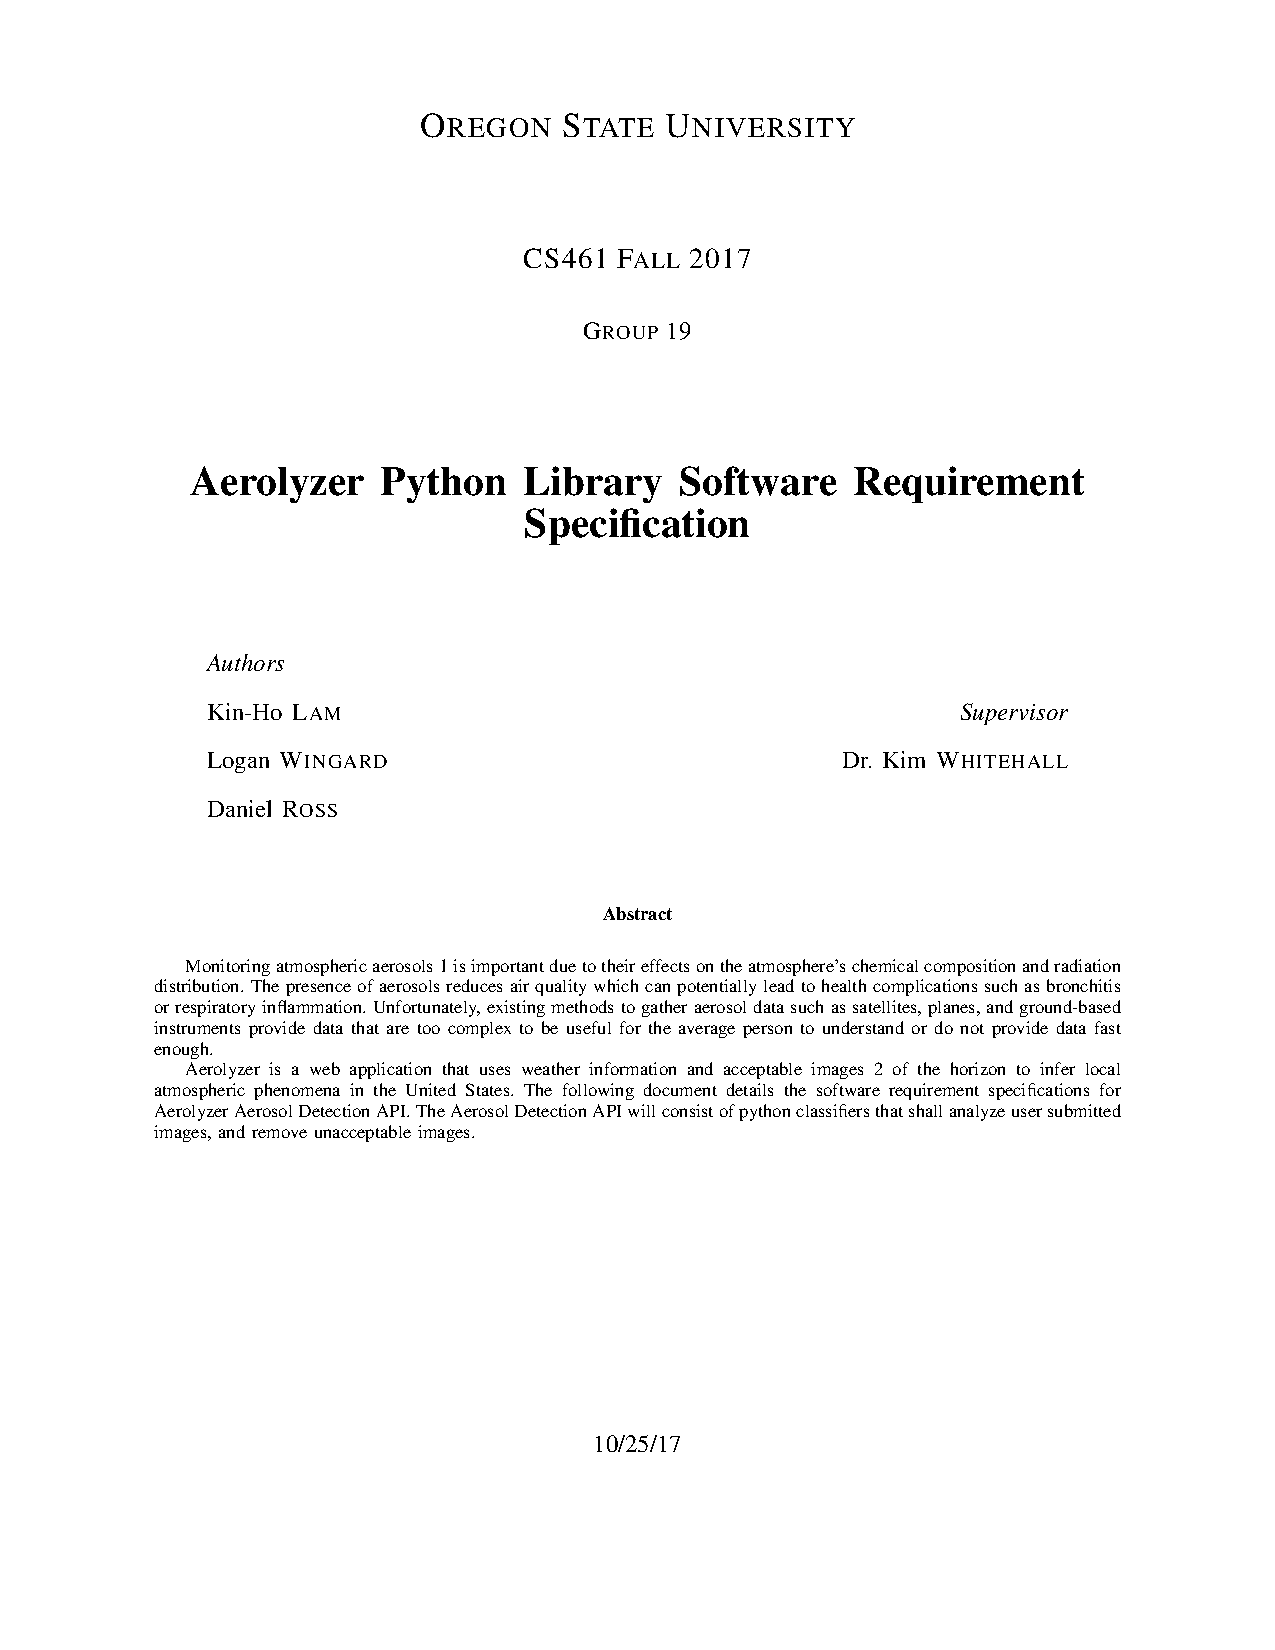
\includepdf[pages=-]{pdfs/require.pdf}
	\section{Design Document}
		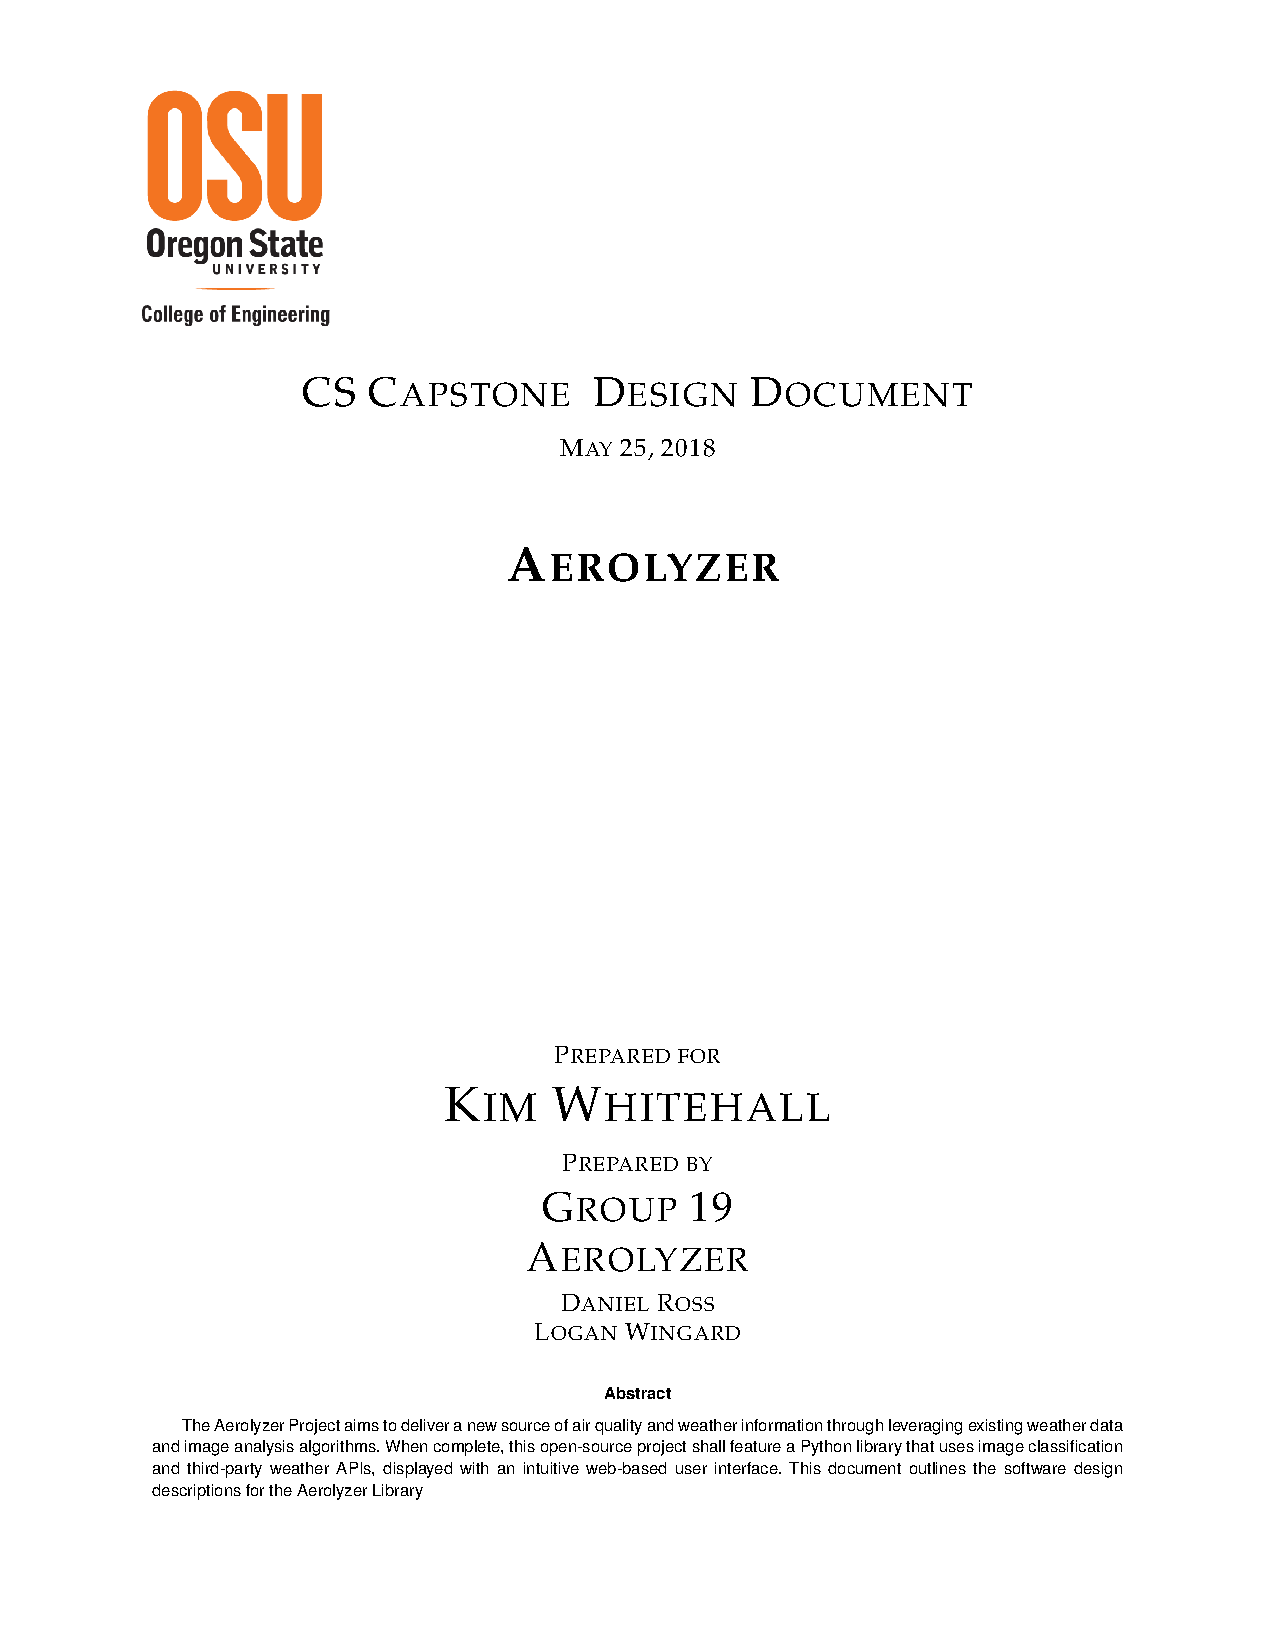
\includepdf[pages=-]{pdfs/design.pdf}
	\section{Tech Review}
		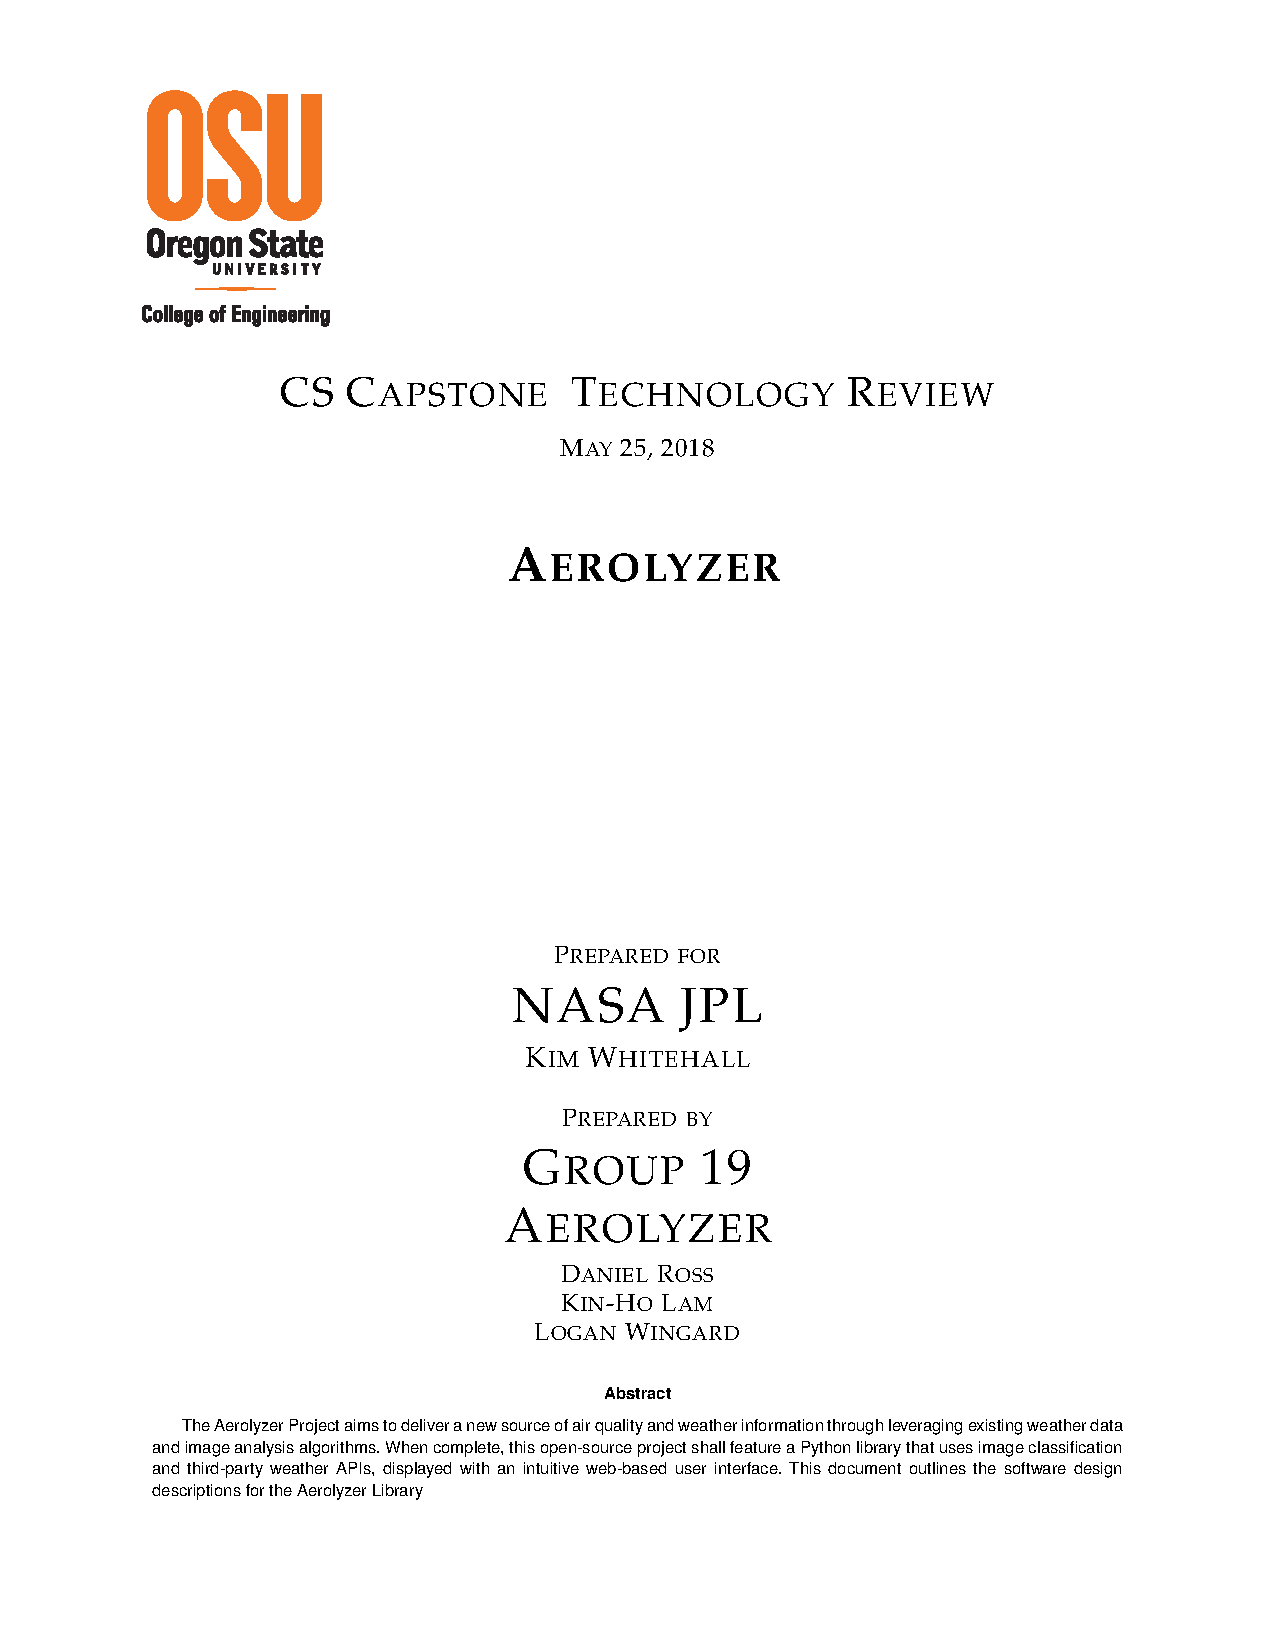
\includepdf[pages=-]{pdfs/tech.pdf}
	\section{Blog Posts}
		\subsection{Daniel Ross}
			todo
		\subsection{Logan Wingard}
			todo
	\section{Poster}
		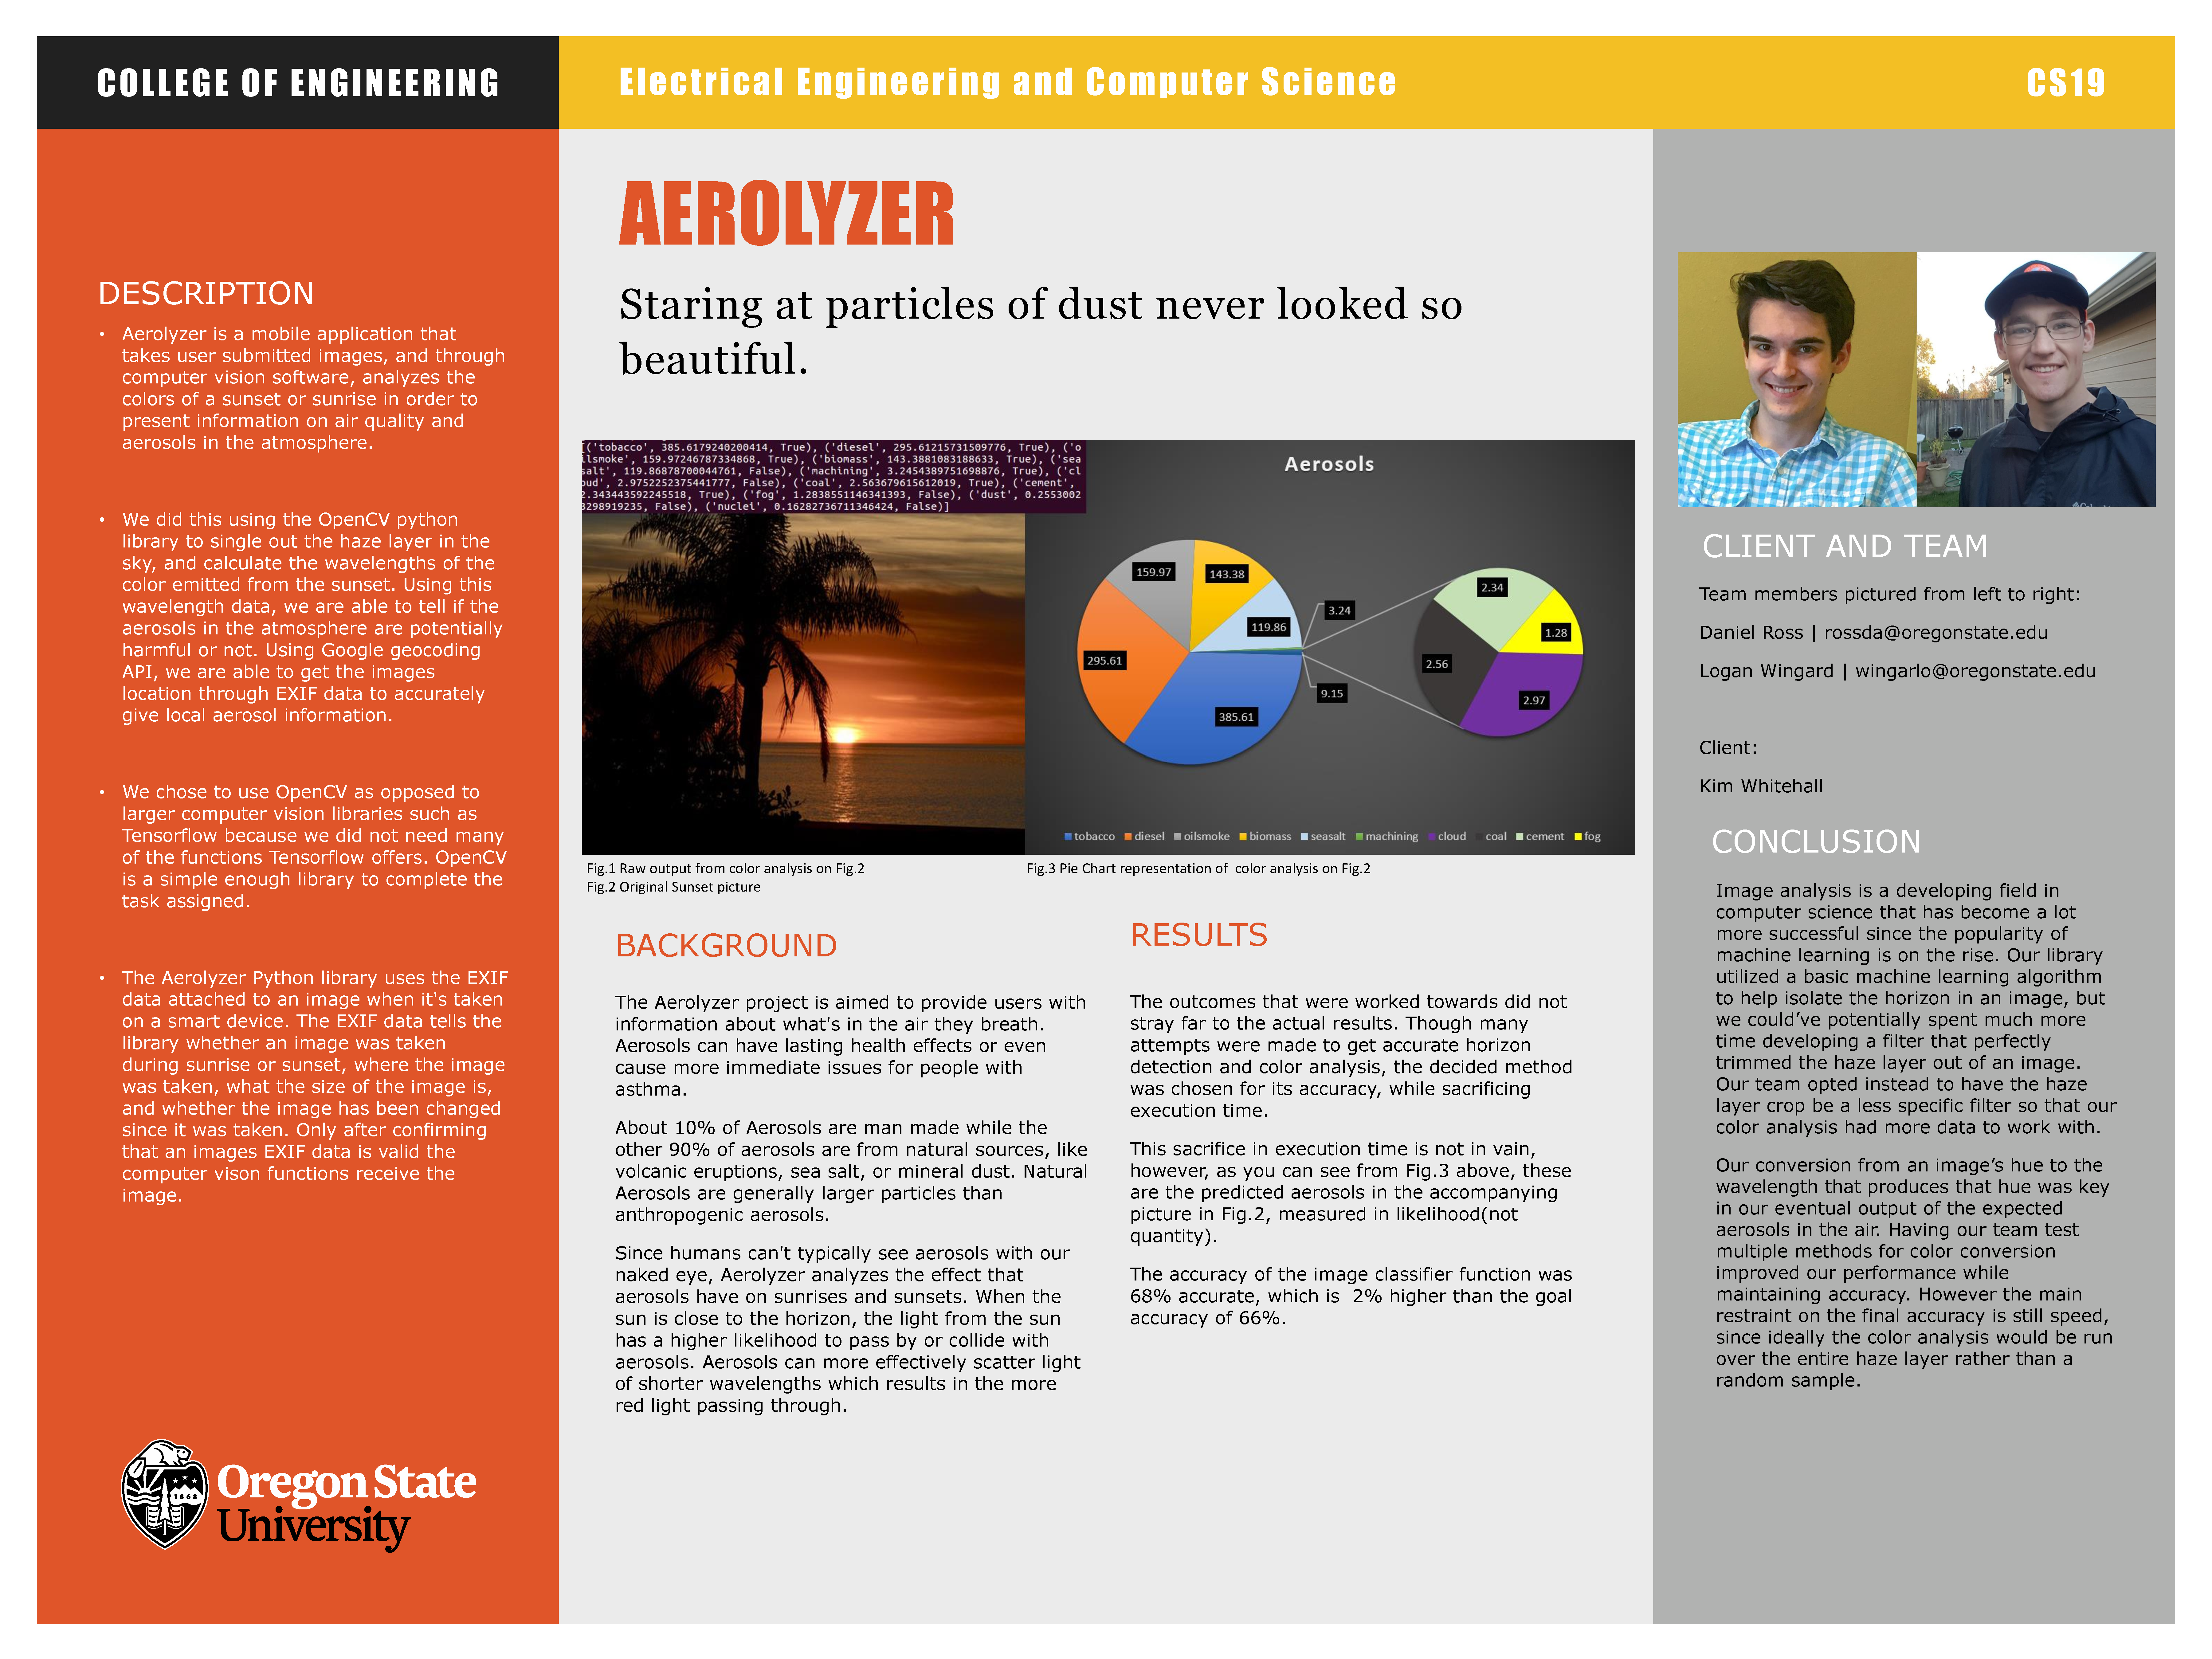
\includepdf[pages=-]{pdfs/poster.pdf}
	\section{Project Documentations}
		todo
	\section{Recommended Resources for Learning More}
		Aerolyzer is completely open source and is even on the Python Package Index (pypi).
		To learn more about how Aerolyzer works, all the code and documentation is on the Aerolyzer github.
		Some of the resources used to learn the techniques implemented into the Aerolyzer library include the following.
		
	\section{Conclusion}
		todo \cite{neural}
	\section{Appendix}
		todo
\end{singlespace}
\clearpage
\bibliographystyle{IEEEtran}
\bibliography{ref}
\end{document}
